
\documentclass[a4paper,11pt]{article}
\usepackage[a4paper, margin=8em]{geometry}

% usa i pacchetti per la scrittura in italiano
\usepackage[french,italian]{babel}
\usepackage[T1]{fontenc}
\usepackage[utf8]{inputenc}
\frenchspacing 

% usa i pacchetti per la formattazione matematica
\usepackage{amsmath, amssymb, amsthm, amsfonts}

% usa altri pacchetti
\usepackage{gensymb}
\usepackage{hyperref}
\usepackage{standalone}

% imposta il titolo
\title{Appunti Fondamenti di Automatica}
\author{Luca Seggiani}
\date{2025}

% disegni
\usepackage{pgfplots}
\pgfplotsset{width=10cm,compat=1.9}

% imposta lo stile
% usa helvetica
\usepackage[scaled]{helvet}
% usa palatino
\usepackage{palatino}
% usa un font monospazio guardabile
\usepackage{lmodern}

% tikz in sans
\tikzset{every picture/.style={/utils/exec={\sffamily}}}

\renewcommand{\rmdefault}{ppl}
\renewcommand{\sfdefault}{phv}
\renewcommand{\ttdefault}{lmtt}

% circuiti
\usepackage{circuitikz}
\usetikzlibrary{babel}

% disponi il titolo
\makeatletter
\renewcommand{\maketitle} {
	\begin{center} 
		\begin{minipage}[t]{.8\textwidth}
			\textsf{\huge\bfseries \@title} 
		\end{minipage}%
		\begin{minipage}[t]{.2\textwidth}
			\raggedleft \vspace{-1.65em}
			\textsf{\small \@author} \vfill
			\textsf{\small \@date}
		\end{minipage}
		\par
	\end{center}

	\thispagestyle{empty}
	\pagestyle{fancy}
}
\makeatother

% disponi teoremi
\usepackage{tcolorbox}
\newtcolorbox[auto counter, number within=section]{theorem}[2][]{%
	colback=blue!10, 
	colframe=blue!40!black, 
	sharp corners=northwest,
	fonttitle=\sffamily\bfseries, 
	title=Teorema~\thetcbcounter: #2, 
	#1
}

% disponi definizioni
\newtcolorbox[auto counter, number within=section]{definition}[2][]{%
	colback=red!10,
	colframe=red!40!black,
	sharp corners=northwest,
	fonttitle=\sffamily\bfseries,
	title=Definizione~\thetcbcounter: #2,
	#1
}

% disponi problemi
\newtcolorbox[auto counter, number within=section]{problem}[2][]{%
	colback=green!10,
	colframe=green!40!black,
	sharp corners=northwest,
	fonttitle=\sffamily\bfseries,
	title=Problema~\thetcbcounter: #2,
	#1
}

% disponi codice
\usepackage{listings}
\usepackage[table]{xcolor}

\lstdefinestyle{codestyle}{
		backgroundcolor=\color{black!5}, 
		commentstyle=\color{codegreen},
		keywordstyle=\bfseries\color{magenta},
		numberstyle=\sffamily\tiny\color{black!60},
		stringstyle=\color{green!50!black},
		basicstyle=\ttfamily\footnotesize,
		breakatwhitespace=false,         
		breaklines=true,                 
		captionpos=b,                    
		keepspaces=true,                 
		numbers=left,                    
		numbersep=5pt,                  
		showspaces=false,                
		showstringspaces=false,
		showtabs=false,                  
		tabsize=2
}

\lstdefinestyle{shellstyle}{
		backgroundcolor=\color{black!5}, 
		basicstyle=\ttfamily\footnotesize\color{black}, 
		commentstyle=\color{black}, 
		keywordstyle=\color{black},
		numberstyle=\color{black!5},
		stringstyle=\color{black}, 
		showspaces=false,
		showstringspaces=false, 
		showtabs=false, 
		tabsize=2, 
		numbers=none, 
		breaklines=true
}

\lstdefinelanguage{javascript}{
	keywords={typeof, new, true, false, catch, function, return, null, catch, switch, var, if, in, while, do, else, case, break},
	keywordstyle=\color{blue}\bfseries,
	ndkeywords={class, export, boolean, throw, implements, import, this},
	ndkeywordstyle=\color{darkgray}\bfseries,
	identifierstyle=\color{black},
	sensitive=false,
	comment=[l]{//},
	morecomment=[s]{/*}{*/},
	commentstyle=\color{purple}\ttfamily,
	stringstyle=\color{red}\ttfamily,
	morestring=[b]',
	morestring=[b]"
}

% disponi sezioni
\usepackage{titlesec}

\titleformat{\section}
	{\sffamily\Large\bfseries} 
	{\thesection}{1em}{} 
\titleformat{\subsection}
	{\sffamily\large\bfseries}   
	{\thesubsection}{1em}{} 
\titleformat{\subsubsection}
	{\sffamily\normalsize\bfseries} 
	{\thesubsubsection}{1em}{}

% disponi alberi
\usepackage{forest}

\forestset{
	rectstyle/.style={
		for tree={rectangle,draw,font=\large\sffamily}
	},
	roundstyle/.style={
		for tree={circle,draw,font=\large}
	}
}

% disponi algoritmi
\usepackage{algorithm}
\usepackage{algorithmic}
\makeatletter
\renewcommand{\ALG@name}{Algoritmo}
\makeatother

% disponi numeri di pagina
\usepackage{fancyhdr}
\fancyhf{} 
\fancyfoot[L]{\sffamily{\thepage}}

\makeatletter
\fancyhead[L]{\raisebox{1ex}[0pt][0pt]{\sffamily{\@title \ \@date}}} 
\fancyhead[R]{\raisebox{1ex}[0pt][0pt]{\sffamily{\@author}}}
\makeatother

\begin{document}

% sezione (data)
\section{Lezione del 10-04-25}

% stili pagina
\thispagestyle{empty}
\pagestyle{fancy}

% testo
Riprendiamo la trattazione dei diagrammi di Bode di funzioni di trasferimento di uso comune.

\subsection{Poli complessi coniugati}
Prendiamo la funzione di trasferimento con denominatore al second'ordine:
$$
G(s) = \frac{1}{1 + \frac{2 \xi}{\omega_0}s + \frac{s^2}{\omega_0^2}}
= \frac{\omega_0^2}{s^2 + 2 \xi \omega_0 s + \omega_0^2}
$$
dove ricordiamo $\omega_0$ è la \textbf{pulsazione naturale} e $\xi$ è lo smorzamento.

Prendiamo quindi la prima forma, che altro non è se non la forma di Bode e ricaviamo la risposta armonica:
$$
G(j \omega) = \frac{1}{1 + \frac{2 \xi}{\omega_0} j \omega - \frac{\omega^2}{\omega_0^2}} = \frac{1}{ \left( 1 - \frac{\omega^2}{\omega_0^2} \right) + j \left( \frac{2 \xi}{\omega_0} \omega \right) }
$$

\subsubsection{Valutazione del modulo}
Troviamo quindi il modulo:
$$
|G(j\omega)| = \frac{1}{ \sqrt{ \left( 1 - \frac{\omega^2}{\omega_0} \right)^2 + 4 \xi^2 \frac{\omega^2}{\omega_0^2} } }
$$
da cui la risposta in decibel:
$$
|G(j \omega)|_{dB} = 20 \log_{10} \left( \frac{1}{ \sqrt{ \left( 1 - \frac{\omega^2}{\omega_0} \right)^2 + 4 \xi^2 \frac{\omega^2}{\omega_0^2} } } \right) 
$$

Possiamo allora tracciare il diagrama a rette prendendo il punto di rottura in $\omega_0$:
\begin{itemize}
	\item $\omega << \omega_0$, da cui:
		$$
			|G(j\omega)| \approx 0 \, \mathrm{dB}
		$$
	\item $\omega >> \omega_0$, da cui:
		$$
			|G(j \omega)| \approx 20 \log \left( \frac{1}{ \frac{\omega^2}{\omega_0^2} } \right) = 40 \log(\omega_0) - 40 \log(\omega)
		$$
		cioè si ottiene una retta con pendenza di -40 dB/dec (-12 dB/oct).
\end{itemize}

\par\bigskip

\noindent
\begin{minipage}{\textwidth}
Da cui si ottiene l'approssimazione (sovraimposta al valore reale):
\begin{center}
	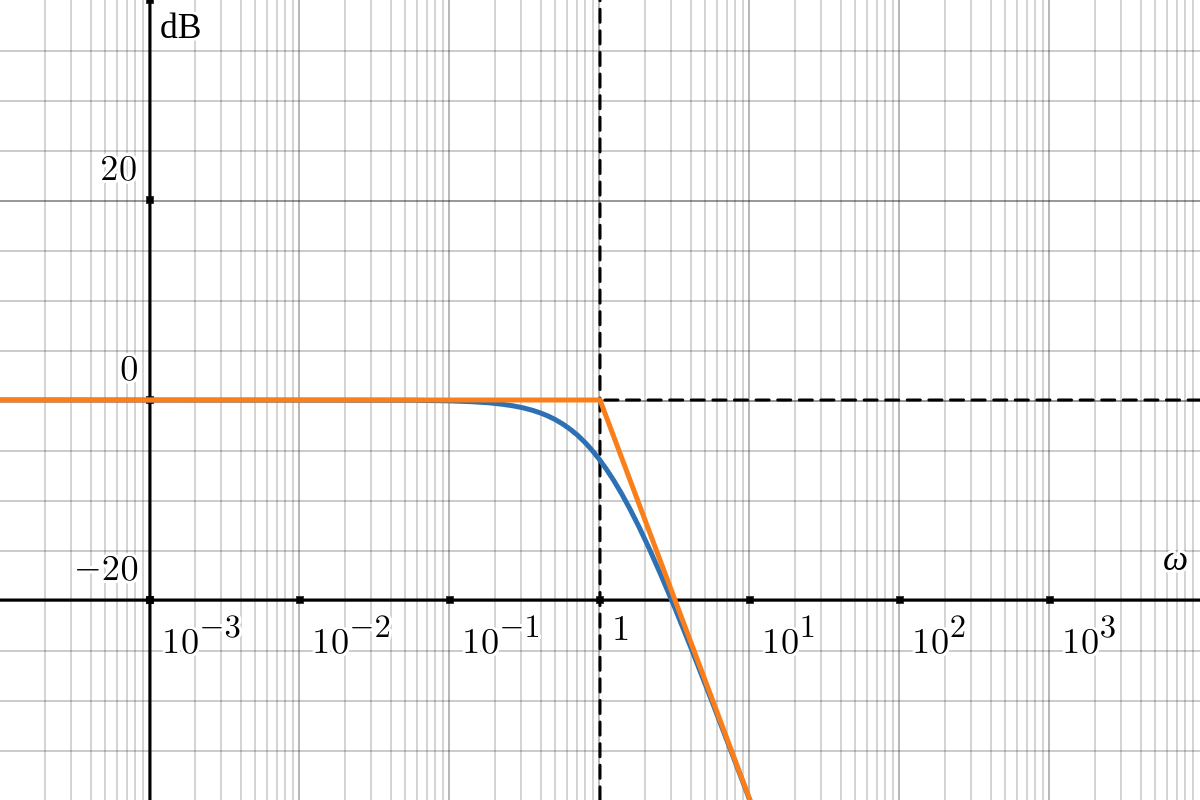
\includegraphics[scale=0.3]{../figures/order2_bode/clean_mod.png}
\end{center}
\end{minipage}

\par\bigskip

\subsubsection{Risonanza}
Potrebbe interessarci valutare l'errore, sopratutto considerato il fatto che non teniamo conto dello smorzamento $\xi$ nella stima per rette.
Prendiamo quindi il valore sul punto di rottura:
$$
|G(j\omega_0)|_{dB} = 20 \log \left( \frac{1}{4 \xi^2} \right) = -20 \log\left( 2 \xi \right) 
$$
per cui si ottengono gli errori al variare di $\xi$ (considerata la nostra approssimazione per rette che prende 0 dB a $\omega = \omega_0$):
\begin{table}[h!]
	\center \rowcolors{2}{white}{black!10}
	\begin{tabular} { c | c }
		$\mathbf{\xi}$ & \bfseries Errore \\ 
		\hline
		$0$ & $+\infty$ \\
		$\frac{1}{2}$ & 0 dB \\
		$\frac{\sqrt{2}}{2}$ & -3 dB \\
		$2$ & -6 dB \\
	\end{tabular}
\end{table}

Come regola empirica, possiamo assumere di poter usare il diagramma asintotico (il diagramma per rette) solo quando lo smorzamento è $\xi > 0.3$.

\par\bigskip

\noindent
\begin{minipage}{\textwidth}
Vediamo ad esempio l'errore che commettiamo per $\xi = \frac{1}{4}$, che calcoliamo subito dovrà essere di 6 dB:

\begin{center}
	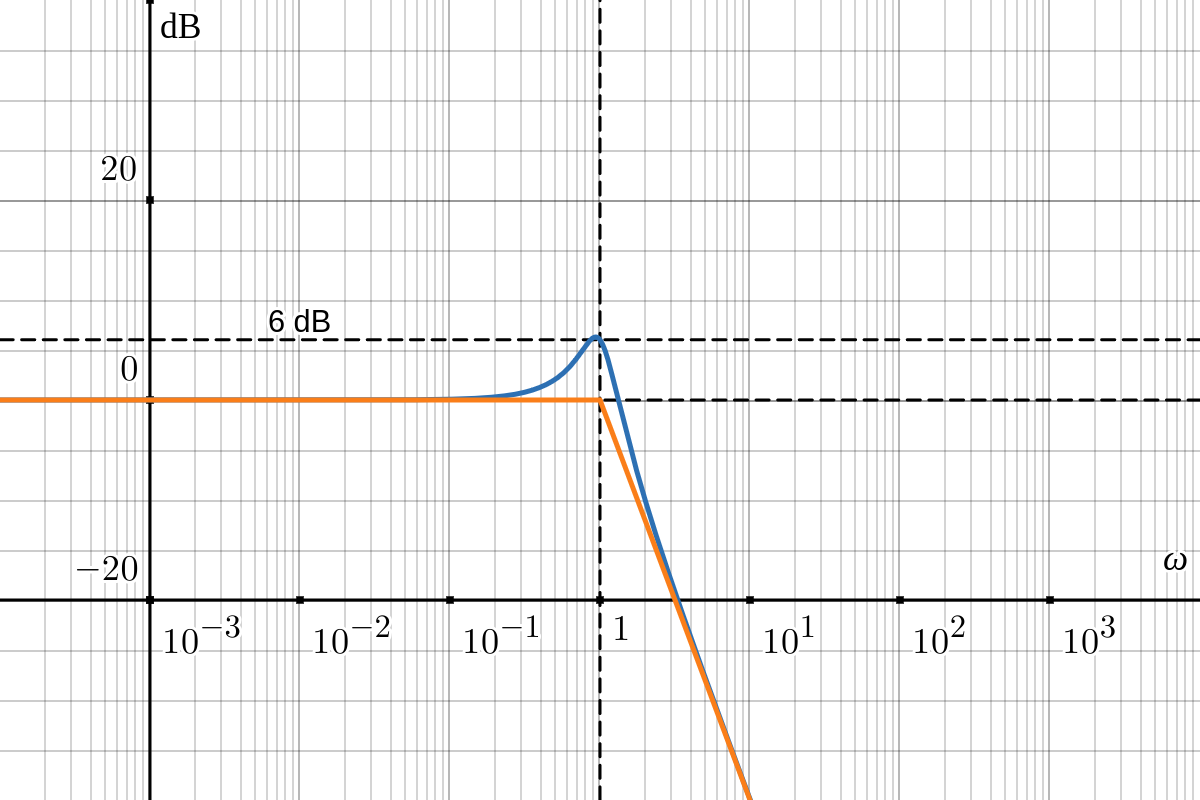
\includegraphics[scale=0.3]{../figures/order2_bode/reso_025_mod.png}
\end{center}
\end{minipage}

\par\bigskip

Come notiamo, si forma un picco attorno a $\omega = \omega_0$, dove la risposta ha un valore di picco vicino (in verità a $\xi$ decrescente il massimo assoluto si sposta sempre più verso sinistra) all'errore calcolato.
Questo picco prende il nome di \textbf{picco di risonanza}.

\subsubsection{Picco di risonanza}
Per ricavare il \textbf{punto di picco} effettivo, cerchiamo il punto stazionario della funzione:
$$
f(u) = (1 - u^2) + 4 \xi^2 u^2, \quad u= \frac{\omega}{\omega_0}
$$
che è il denominatore del modulo.

Abbiamo quindi, derivando:
$$
\frac{d}{du} f(u) = 0 = -4u(1 - u^2) + 8 \xi^2 u
$$
da cui:
$$
u_{max} = \frac{\omega_{max}}{\omega_0} = \sqrt{1 - 2 \xi^2}
$$
cioè il \textit{punto di picco} è:
$$
\omega_{max} = \omega_0 \sqrt{1 - 2 \xi^2} 
$$
e il \textit{valore di picco}, ovvero il modulo in decibel raggiunto nel punto di picco, è pari a:
$$
\max |G(j \omega)|_{dB} = 20 \log \left( |G(\omega_{max})| \right)
$$
Osserviamo che questo valore è effettivamente definito su $\mathbb{R}$ solo quando $\xi < \frac{1}{\sqrt{2}}$: questo si spiega semplicemente dal fatto che per $\xi > \frac{1}{\sqrt{2}}$ la funzione modulo del trasferimento è monotona, e non esiste nessun picco.

\par\bigskip

\noindent
\begin{minipage}{\textwidth}
Vediamo quindi il punto di picco dell'esempio precedente, dove ricordiamo avevamo preso $\xi = \frac{1}{4}$:

\begin{center}
	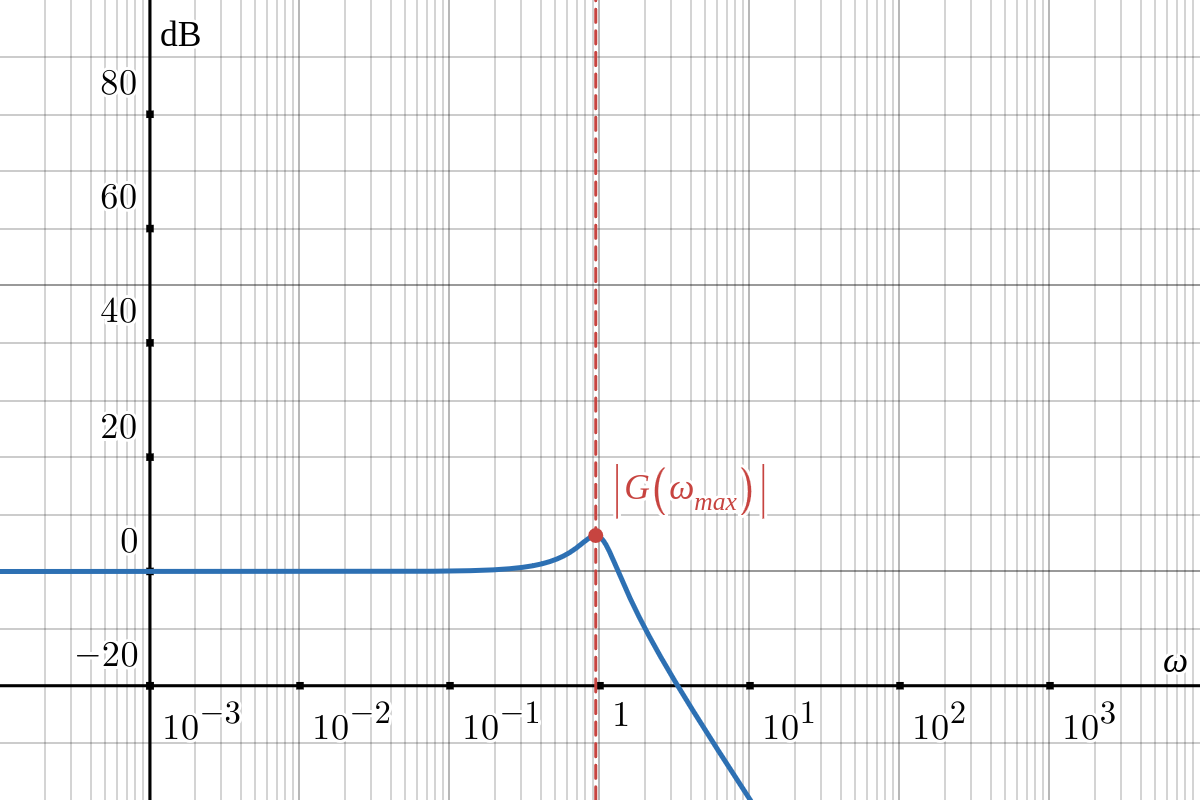
\includegraphics[scale=0.3]{../figures/order2_bode/peak_point.png}
\end{center}
\end{minipage}

\par\bigskip

Il valore $\omega_{max}$, calcolato al computer, risulta circa $\sim 0.935$, per cui l'errore $\left| G \left( \omega_{max} \right) \right|$ in questo caso è abbastanza vicino all'errore in $\omega = 1$, che era di 6 dB.

\par\bigskip

\noindent
\begin{minipage}{\textwidth}
Possiamo quindi riportare un grafico che mostra la variazione del picco di risonanza al variare dello smorzamento $\xi$:

\begin{center}
	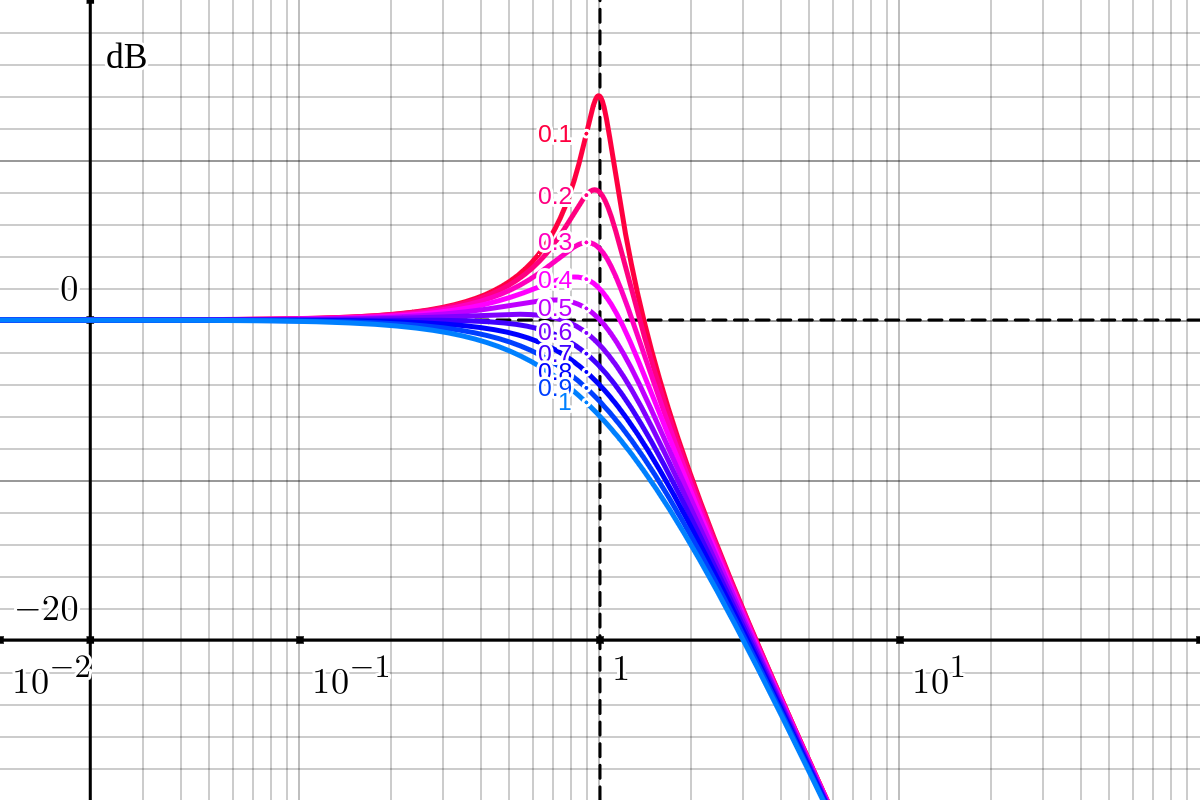
\includegraphics[scale=0.3]{../figures/order2_bode/peak_plot.png}
\end{center}
\end{minipage}

\par\bigskip

Questo grafico è duale a quello in 14.1.1: prima avevamo parlato della risposta a transiente, e adesso parliamo della risposta a regime, ma in entrambi i casi vediamo favorire una certa frequenza di oscillazione $\omega_0$ (che nel transiente avevamo visto è corretta di un fattore dipendente dallo smorzamento).

Inoltre, si vede molto bene come intorno a $0.7 \approx \frac{1}{\sqrt{2}}$ il picco scompare: questa è la conseguenza diretta del fatto che, come abbiamo detto, il punto di picco $\omega_0 \sqrt{1 - 2 \xi^2}$ è effettivamente definito su $\mathbb{R}$ solo nel caso $\xi < \frac{1}{\sqrt{2}}$.

\par\smallskip

Facciamo quindi un breve riassunto sulle frequenze di oscillazione che abbiamo incontrato finora:
\begin{itemize}
	\item \textbf{Frequenza di oscilazione naturale:} $\ \omega_0$ \\
		Abbiamo detto sarebbe la frequenza naturale a cui il sistema oscillasse se non vi fosse smorzamento $\xi$, e infatti vediamo che in tal caso corrisponde esattamente alle altre 2 frequenze; 
	\item \textbf{Frequenza di oscillazione naturale smorzata:} $\ \omega_d = \omega_0 \sqrt{1 - \xi^2}$ \\
		Rappresenta la frequenza di oscillazione della \textit{risposta libera} del sistema, cioè quella con cui, nel caso questo sia stabile, decade naturalmente al punto di equilibrio (l'origine); 
	\item \textbf{Frequenza di picco risonante:} $\ \omega_{max} = \omega_0 \sqrt{1 - 2 \xi^2}$ \\
		Rappresenta ciò che abbiamo appena visto, cioè la frequenza che il sistema, preso dal punto di vista della funzione di trasferimento ingresso-uscita, amplifica più delle altre (sotto l'ipotesi $\xi < \frac{1}{\sqrt2}$). In questo è intrinsecamente legata alla \textit{risposta forzata} del sistema.
\end{itemize}

Si ricava immediatamente che nei sistemi sottosmorzati $\xi < 1$ (che sono comunqe gli unici dove questo tipo di considerazioni si applicano), vale fra queste frequenze la relazione:
$$
\omega_{max} < \omega_d < \omega_0
$$
cioè il sistema preferisce oscillare, in \textit{risposta libera} ($\omega_d$), ad una frequenza leggermente più alta di quella di eccitazione massima in \textit{risposta forzata} ($\omega_{max}$).

\subsubsection{Valutazione di fase}
Per quanto riguarda la fase, invece, si avrà: 
$$
\angle G(j \omega) = -\mathrm{atan2} \left( \frac{ \frac{2\xi}{\omega_0}\omega }{ 1 - \frac{\omega^2}{\omega_0^2} } \right) 
$$
in quanto l'unico termine che determina la fase è il denominatore.

Potremo quindi prendere l'approssimazione per rette:
\[
	\begin{cases}
		\omega << \omega_0 \implies \angle G(j\omega) \approx 0^\circ \\ 	
		\omega >> \omega_0 \implies \angle G(j\omega) \approx -180^\circ \\ 	
		\omega = \omega_0 \implies \angle G(j\omega) = -90^\circ \\ 	
	\end{cases}
\]
preso $\tau > 0$.

Il valore in $\omega = \omega_0$ si calcola osservando che:
$$
\angle G(j \omega_0) = -\mathrm{atan2} \left( \frac{ 2 \xi }{ 0^+ } \right)
$$
da cui il limite, che porta appunto a $-90^\circ$.

\par\bigskip

\noindent
\begin{minipage}{\textwidth}
Otteniamo quindi il grafico approssimato, come sempre sovraimposto a quello reale:

\begin{center}
	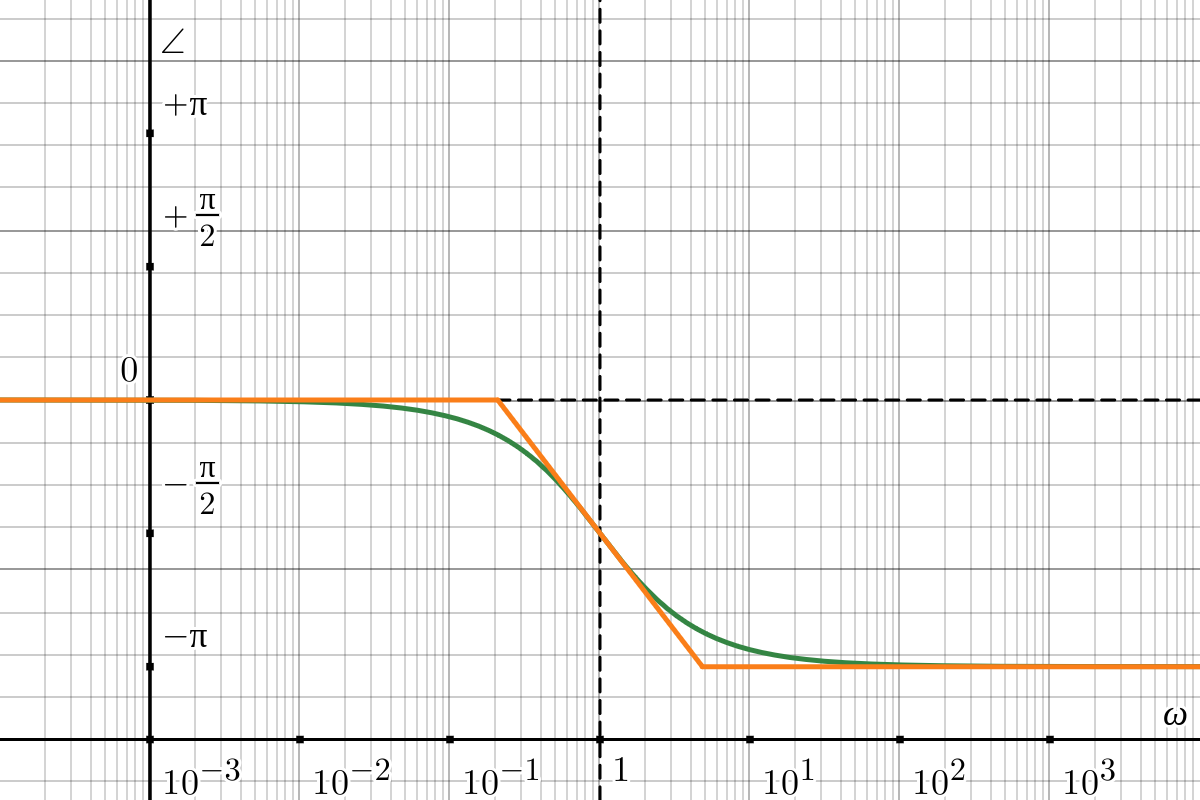
\includegraphics[scale=0.3]{../figures/order2_bode/phase.png}
\end{center}
\end{minipage}

\par\bigskip

Vediamo che lo scostamento in fase è lo stesso del sistema del primo ordine, ma raddoppiato: questo ha senso, in quanto abbiamo detto già lo stesso abbattimento dopo la frequenza di taglio $\omega_0$ era del doppio, cioè -40 dB/dec.

\par\smallskip

Una considerazione più interessante potrebbe essere quella della pendenza della retta che approssima la componente intorno a $\omega_0$: abbiamo infatti che, a differenza dei sistemi del prim'ordine, nei sistemi del second'ordine lo scostamento in fase avviene con velocità diverse intorno alla frequenza di taglio (finora si è assunto $-1$): è proprio questo a dare il caratteristico picco di risonanza (rispettate le condizioni di cui sopra).

Calcoliamo allora la derivata dell'argomento della risposta:
$$
\frac{d}{d\omega} \left( \angle G(j\omega) \right) 
= - \frac{1}{1 + \left( \frac{ \frac{2 \xi \omega}{\omega_0} }{ 1 - \frac{\omega^2}{\omega_0^2} } \right)^2 } 
\cdot \frac{ \frac{2 \xi}{\omega_0} \left( 1 - \frac{\omega^2}{\omega_0^2} \right) + \frac{2 \xi \omega}{\omega_0} \cdot \frac{2 \omega}{\omega_0^2} }{ \left( 1 - \frac{\omega^2}{\omega_0^2} \right)^2 }
$$
Questa funzione, valutata in $\omega_0$, dà:
$$
\frac{d}{d\omega} \left( \angle G(j\omega) \right) (j \omega_0) = - \frac{2 \xi}{\omega_0} \cdot \frac{ \left( 1 + \frac{\omega_0^2}{\omega_0^2} \right) }{ \left( 1 - \frac{\omega_0^2}{\omega_0^2} \right)^2 + \left( \frac{2 \xi \omega_0}{\omega_0} \right)^2 } = - \frac{1}{\xi \omega_0}
$$
Tracceremo quindi la retta di congiunzione in $\omega = \omega_0$ con coefficiente angolare $- \frac{1}{\xi \omega_0}$.

\par\bigskip

\noindent
\begin{minipage}{\textwidth}
Vediamo ad esempio il caso con $\xi = 0.6$:

\begin{center}
	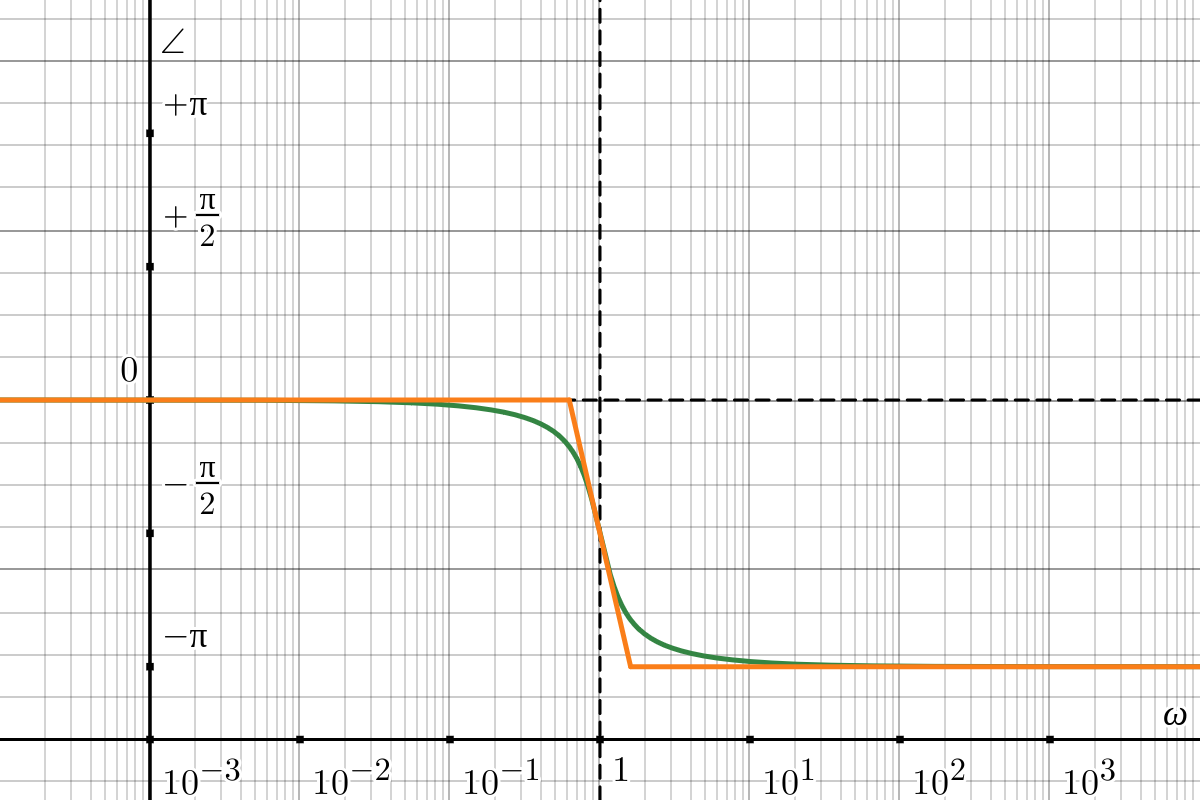
\includegraphics[scale=0.3]{../figures/order2_bode/phase_weird.png}
\end{center}
\end{minipage}

\par\bigskip

Dal punto di vista pratico, possiamo fare la stessa ipotesi di approssimazione di prima: per $\xi > 0.3$ prendiamo la retta con derivata $-1$, mentre per $\xi < 0.3$ la pendenza è troppo ripida perchè questa sia valida.

\subsection{Ritardo nei diagrammi di Bode}
Vediamo infine l'effetto che il ritardo ha nel dominio frequenze.
Avevamo già visto l'espressione del ritardo nel dominio d Laplace:
$$
G(s) = e^{-s \tau}
$$
In risposta armonica, questa dà:
$$
G(j \omega) = e^{-j \omega \tau}
$$
cioè uno scostamento in fase di $\omega \tau$.

L'effetto sul diagramma di Bode sarà quindi di lasciare invariato il modulo (cioè dare una costante a 0 dB), e sopratutto di scostare la fase di un valore pari a $-\omega \tau$.

\par\bigskip

\noindent
\begin{minipage}{\textwidth}
Vediamo allora il grafico del modulo:

\begin{center}
	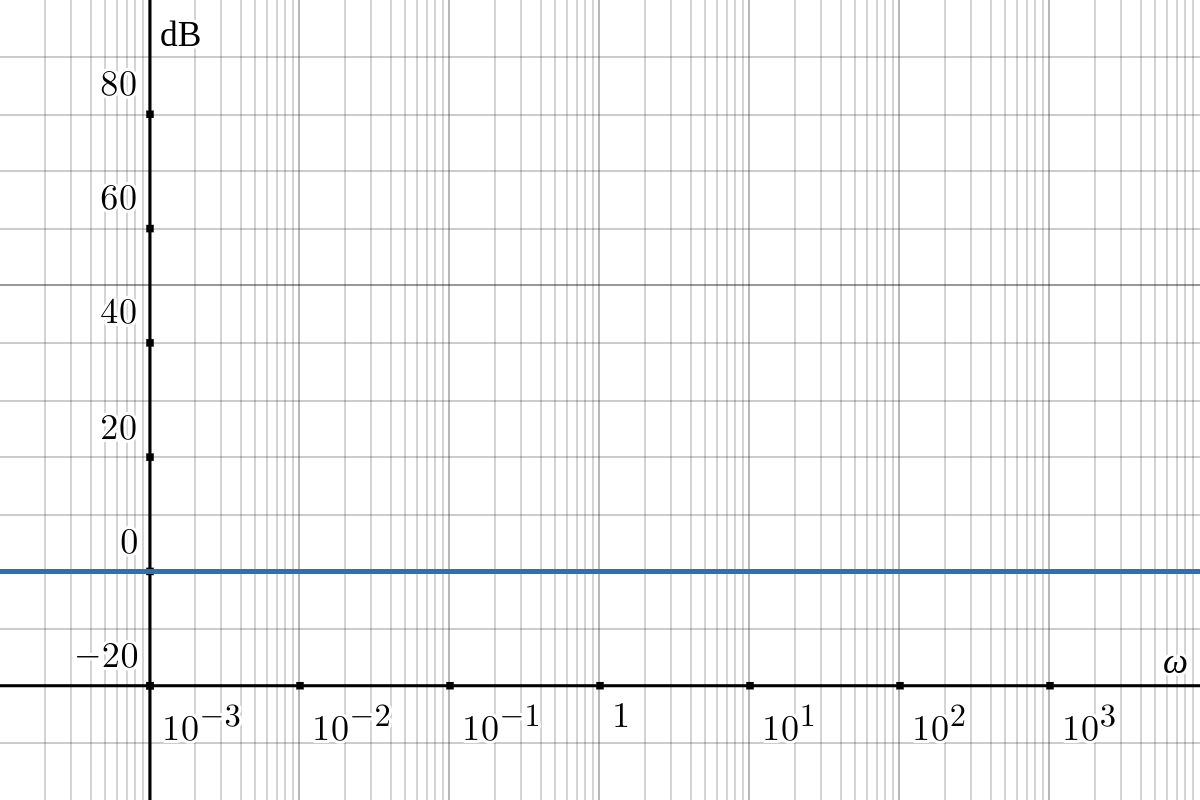
\includegraphics[scale=0.3]{../figures/delay_bode/mod.png}
\end{center}
\end{minipage}

\par\bigskip

\noindent
\begin{minipage}{\textwidth}
e il grafico della fase:

\begin{center}
	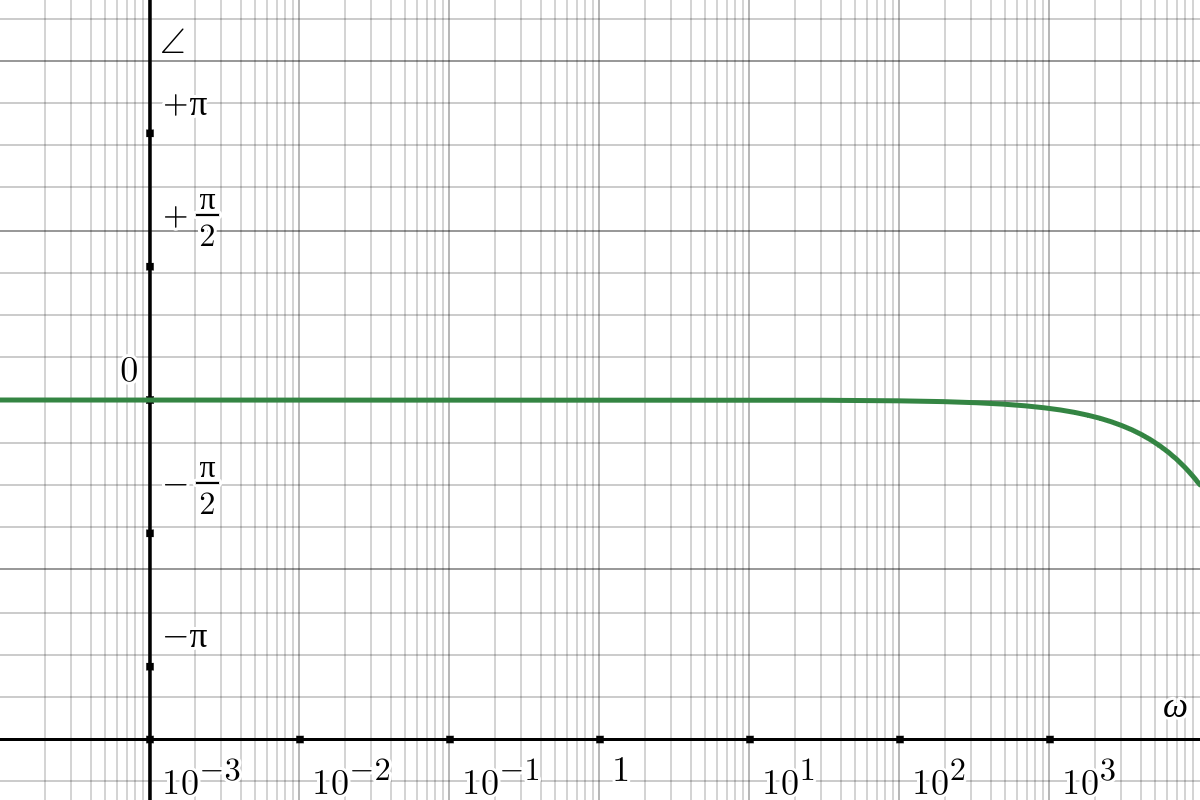
\includegraphics[scale=0.3]{../figures/delay_bode/phase.png}
\end{center}
\end{minipage}

\par\bigskip

\subsection{Esempio: diagramma di Bode}
Vediamo quindi un esempio pratico di disegno di un diagramma di Bode.
Prendiamo la funzione di trasferimento:
$$
G(s) = 200 \frac{\left( s+ \frac{1}{10} \right)}{ (s + 1) \left( \frac{s^2}{400} + \frac{s}{20} + 1 \right) }
$$
che protiamo subito nella forma di Bode e in risposta armonica:
$$
= 20 \frac{\left( 10s + 1 \right)}{ (s + 1) \left( \frac{s^2}{400} + \frac{s}{20} + 1 \right) } 
= 20 \frac{\left( 10 j \omega + 1 \right)}{ (j \omega + 1) \left( -\frac{\omega^2}{400} + \frac{j \omega}{20} + 1 \right) }
$$

Vediamo poi il guadagno: questo nella forma di Bode è dato dal $20$ che moltiplica il rapporto polinomi.
Dalla tabella in 17.2.1 ricordiamo che un modulo di $|20|$ corrisponde a un guadagno di 26 dB.
Aggiugneremo quindi questo valore a tutti i moduli che calcoleremo.

Da qui distinguiamo zeri e poli e ne individuiamo il comportamento tramite un approssimazione per rette.
Da quanto avevamo dimostrato nella 17.1.3, potremo poi sommare i grafici ottenuti dalle singole risposte per zero e per polo e ottenere la risposta complessiva.

Abbiamo quindi:
\begin{itemize}
	\item \textbf{Zeri:}
		\begin{itemize}
			\item $10 j \omega + 1$: questo rappresenta una rampa, con pendenza di 20 dB/dec, che inizia a pulsazione $j \omega^* = \frac{1}{10}$. \\ 
				Dal punto di vista della fase rappresenterà una transizione da $0^\circ$ a $90^\circ$ con punto a derivata unitaria in $\frac{1}{10}$.
		\end{itemize}
	\item \textbf{Poli:}
		\begin{itemize}
			\item $j \omega + 1$: questo rappresenta un passa basso, con pendenza di -20 dB/dec e frequenza di taglio a $j \omega^* = 1$. \\ 
				Dal punto di vista della fase rappresenterà una transizione da $0^\circ$ a $-90^\circ$ con punto a derivata unitaria in $1$;
			\item $-\frac{\omega^2}{400} + \frac{j \omega}{20} + 1$: questa è una forma del secondo grado, di cui ci interessa prima di tutto conoscere il tipo.
				Riconosciamo allora di poterci ricondurre alla forma $-\frac{\omega^2}{\omega_0^2} + \frac{2\xi}{\omega_0} j \omega + 1$, cioè:
				$$
				-\frac{\omega^2}{400} + \frac{j \omega}{20} + 1 = -\frac{\omega^2}{\omega_0^2} + \frac{2\xi}{\omega_0} j \omega + 1
				$$
				da cui:
				$$
				\omega_0^2 = 400 \implies \omega_0 = 20, \quad \frac{2\xi}{\omega_0} = \frac{2\xi}{20} = \frac{1}{20} \implies \xi = \frac{1}{2}
				$$
				cioè siamo nel caso sottosmorazato, tra con l'altro $\xi = 0.5$, che è compreso fra $0.3$ e $0.7$, quindi abbiamo detto \textit{risonante} ma \textit{approssimabile} col diagramma a rette.
				Ignoriamo quindi lo smorzamento e prendiamo un filtro passa basso con pendenza di -40 dB/dec e frequenza di taglio a $j \omega^* = 20$. \\ 
				Dal punto di vista della fase rappresenterà una transizione da $0^\circ$ e $-90^\circ$
		\end{itemize}
\end{itemize}

Tracciamo quindi il diagramma di Bode del modulo, considerando le seguenti regioni:
\begin{itemize}
	\item $[0, 0.1)$: nessun zero o polo è attivo, quindi si resta a 0 + 26 dB;
	\item $[0.1, 1)$: lo zero è attivo, si sale con 20 dB/dec fino a 20 + 26dB;
	\item $[1, 20)$: il polo lineare è attivo e compensa lo zero, si resta a 20 + 26 dB;
	\item $[20, +\infty)$: il polo quadratico è attivo, si scende con -40 db/dec.
\end{itemize}

\par\bigskip

\noindent
\begin{minipage}{\textwidth}
da cui il grafico:

\begin{center}
	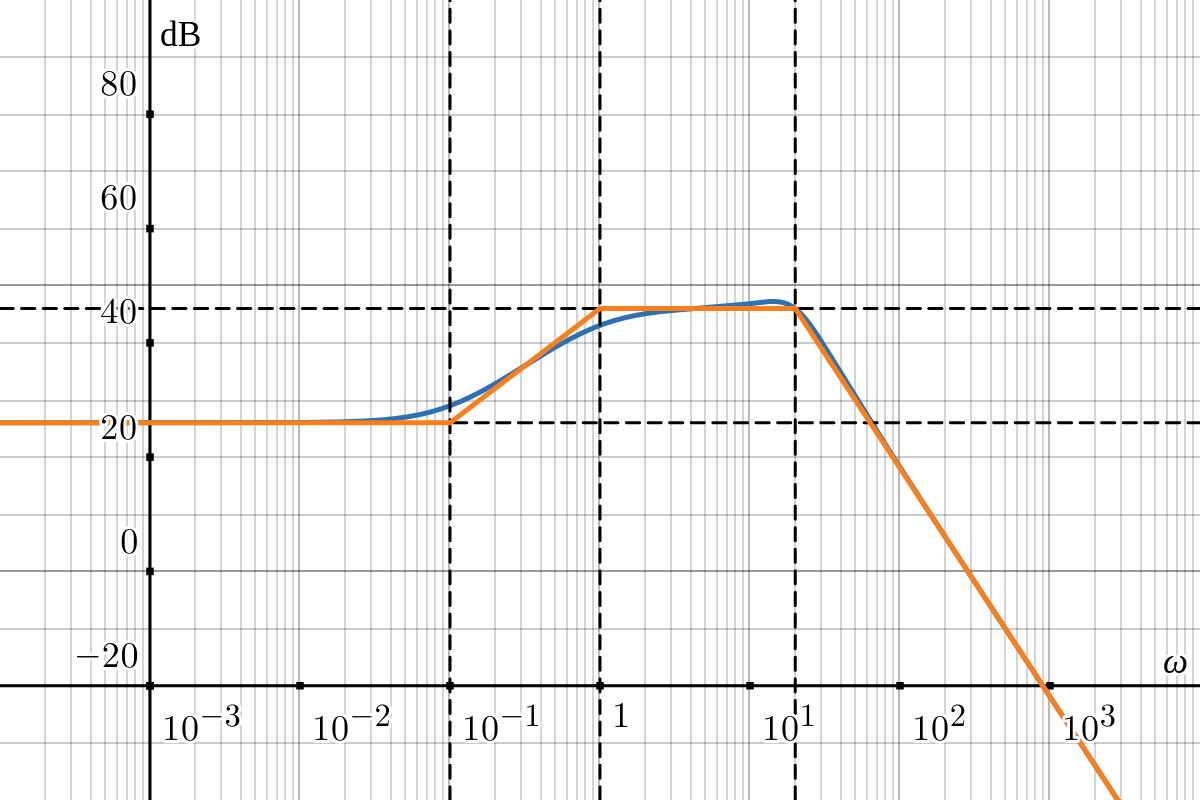
\includegraphics[scale=0.3]{../figures/exerc_bode.png}
\end{center}
\end{minipage}

\par\bigskip

che come vediamo si discosta dal grafico originale per lo più per lo smussamento intorno a $0.1 \sim 1$, e per il picco di risonanza (che abbiamo volontariamente ignorato) a $20$.

\par\smallskip

Disegnamo quindi il diagramma di Bode della fase.
In questo caso notiamo di avere molta sovrapposizione fra le transizioni di fase: un'idea potrebbe essere quella di considerare assoluti solo i valori agli estremi $0$ e a $+\infty$, e per gli zeri e i poli intermedi prendere i punti "medi" (a $\pm 45^\circ$ per lo zero e il polo lineare, e a $-90^\circ$ per il polo quadratico).

\par\bigskip

\noindent
\begin{minipage}{\textwidth}

\begin{center}
	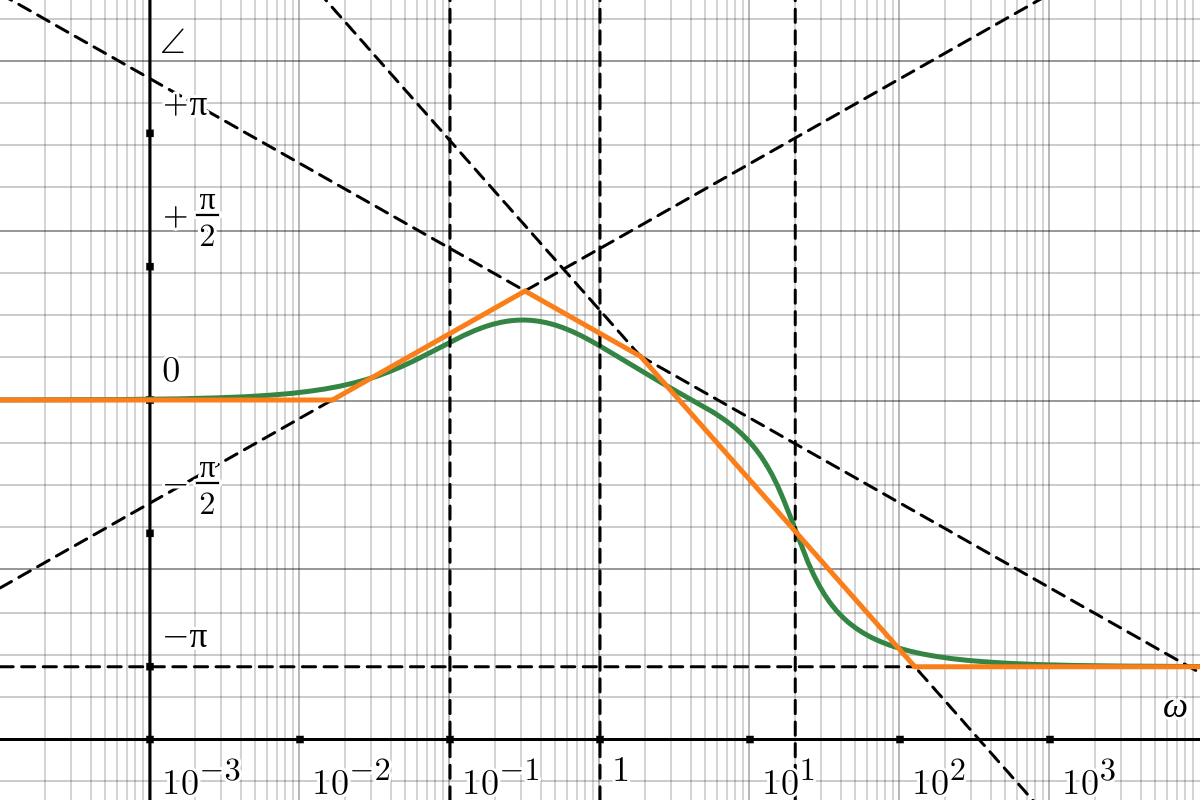
\includegraphics[scale=0.3]{../figures/exerc_bode_phase.png}
\end{center}
\end{minipage}

\par\bigskip

che vediamo essere abbastanza simile alla fase effettiva (in verde).

\end{document}
